\chapter{Introduction}

\section{Motivation}
Logic circuits underpin practically every aspect of modern life in the form of computer chips. It is therefore important that as many people as possible have the opportunity to learn about and understand logic circuits.

The best workbenches I could find on the Internet were Logic.ly\footnote{http://logic.ly} and CircuitLab\footnote{http://www.circuitlab.com}. Even they had problems such as overly simplistic simulations, overly complicated user interfaces, or requiring the need for trusting or installing their program.

I wanted to build a logic circuit workbench which was very simple to access and use, but without simplifying the simulation to the point where it is unhelpful. As modern browsers go to great lengths sandbox a website's JavaScript programs from the user's system, there is no need for the users to trust my implementation to use it.

\section{Overview of GatePlay}
The main interface of GatePlay can be seen in figure~\ref{fig:interface}. The labelled regions are:

\begin{itemize}
	\item[1] The \textbf{top bar} has buttons to download the workbench as an image and to start simulating the circuit.When simulating, the top bar has additional controls such as starting, restarting, and pausing the simulation.
	\item[2] The \textbf{left bar} has sliding panels which contain components available to build circuits with. The user simply drags a gate from the left bar onto the workbench to add it to the circuit.
	\item[3] The \textbf{workbench} is where almost all interaction with GatePlay happens. When editing you can move, delete, and draw wires between components. When simulating the values of wires are shown visually on the workbench.
\end{itemize}

Figure~\ref{fig:dflopflop} shows a D flip-flop being simulated on the workbench. Green wires are $High$ (logical $True$) and red wires are $Low$ (logical $False$). The round components on the left are $Toggle$s; clicking them will change their value and cause the resulting changes to propagate through the circuit.

\begin{figure}[p]
    \centering
    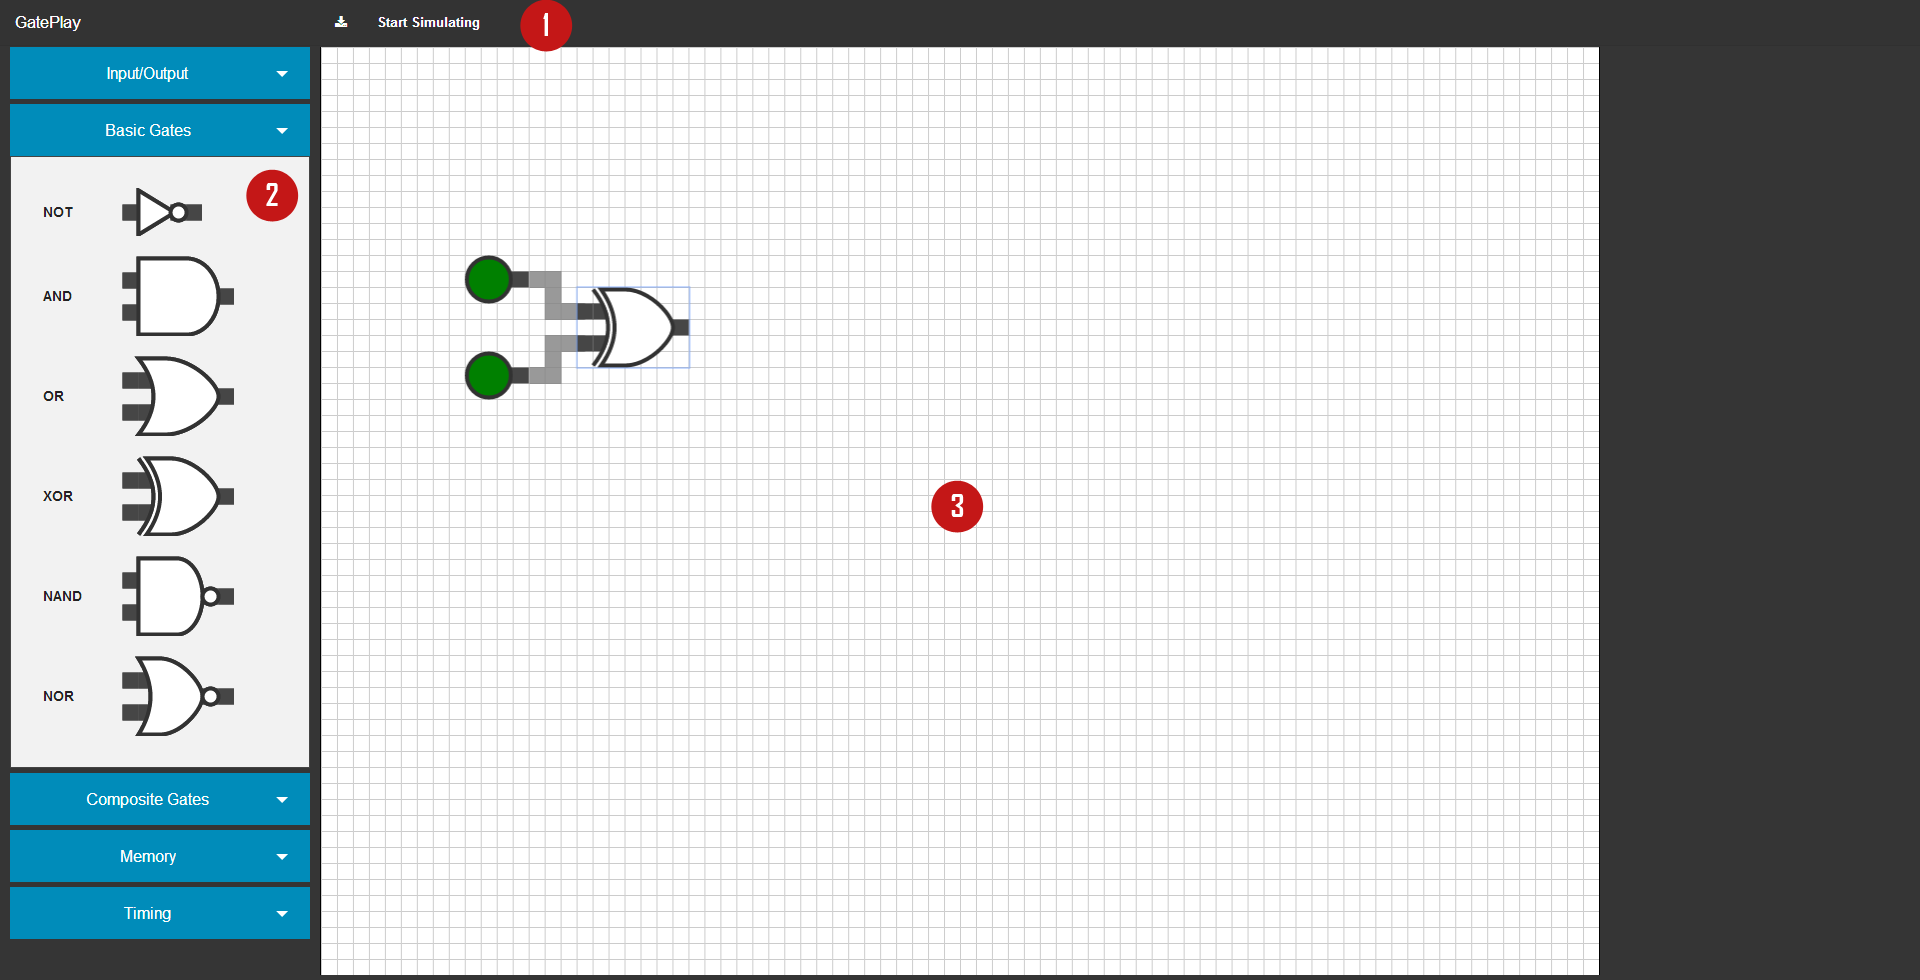
\includegraphics[width=\textheight,angle=90]{labelled.png}
    \caption{Drawing a circuit}
    \label{fig:interface}
\end{figure}

\begin{figure}[p]
    \centering
    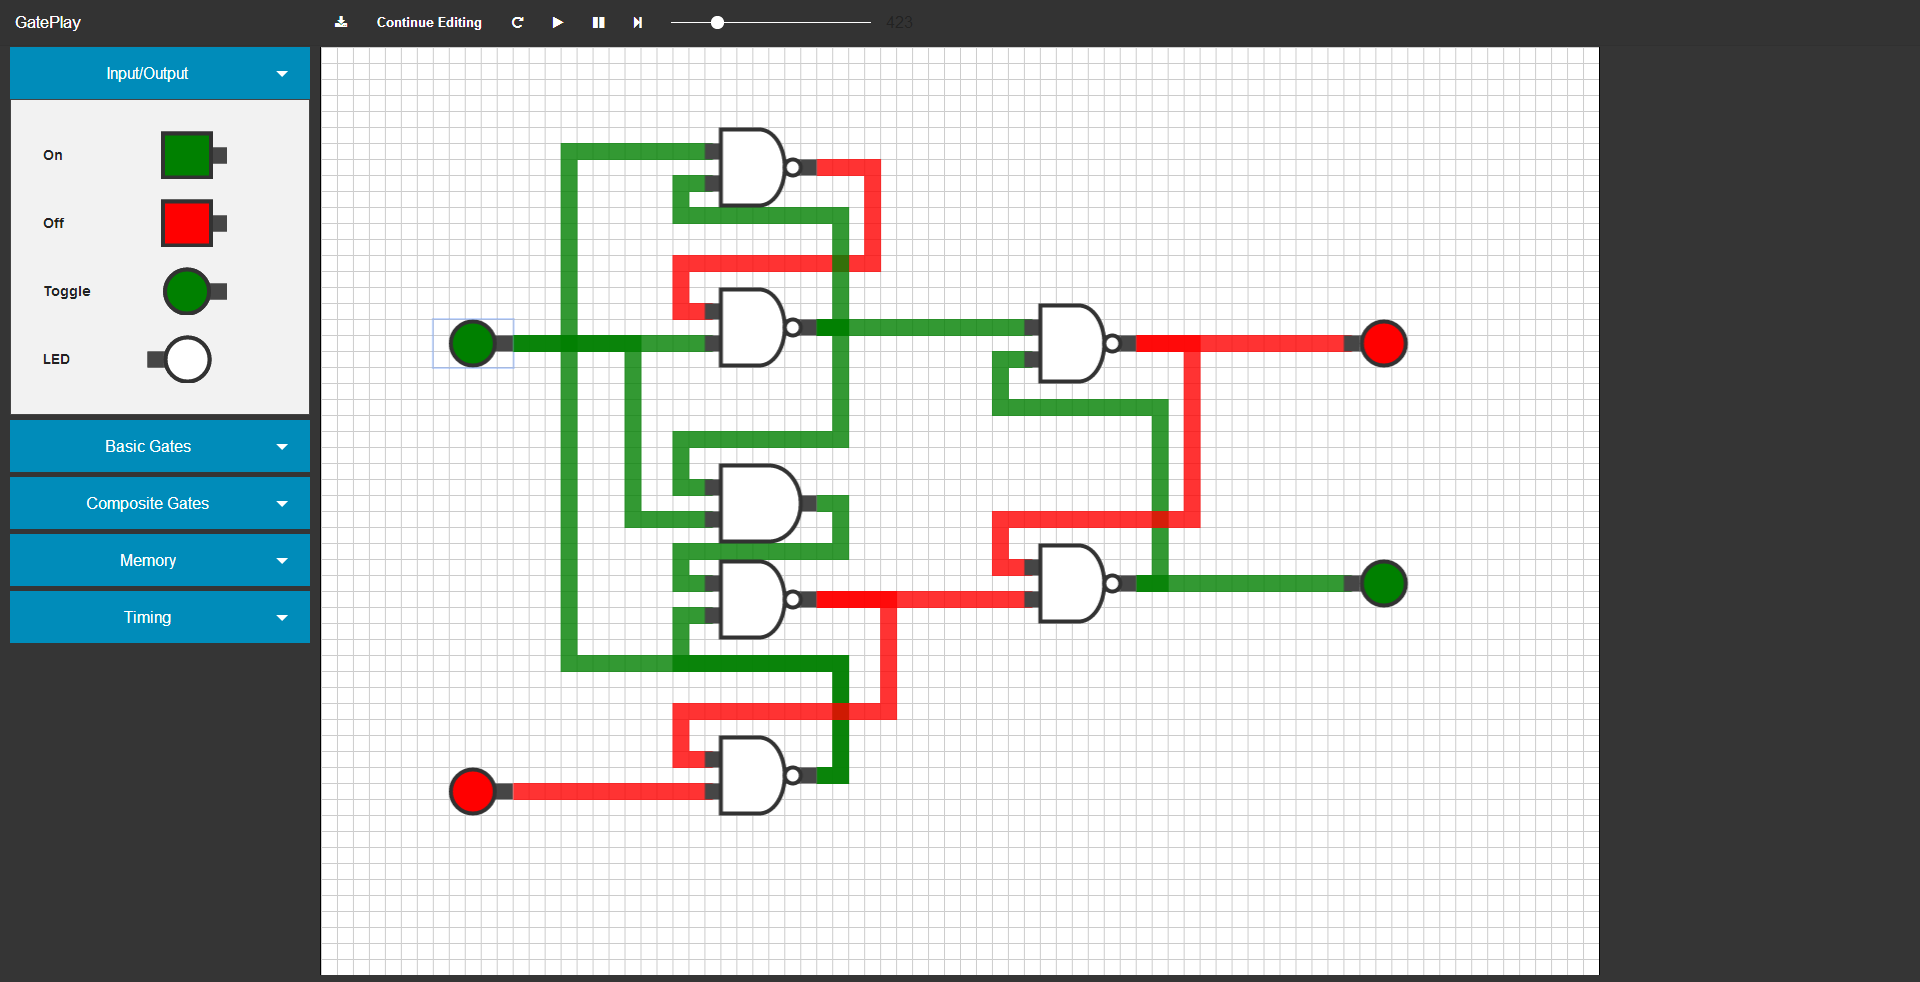
\includegraphics[width=\textheight,angle=90]{dflipflop.png}
    \caption{Simulating a D flip-flop}
    \label{fig:dflopflop}
\end{figure}